\section{Результаты симуляций}

В одном из запусков тестового измерения, описанного в главе~\ref{sec:timeTestsGSI}, источник отсутствовал. Поэтому, записанные сигналы порождались космическими лучами, случайными фотонами, проникшими через стенки чёрного ящика, и шумовыми одноэлектронными сигналами. Уровень триггера, определяющий условие записи сигнала был установлен достаточно низко, чтобы одноэлектронные шумовые сигналы преодолели этот порог. С помощью анализа форм одноэлектронных шумовых сигналов был определен параметр $b$ функции~\eqref{eq:1electronSIM}, характеризующий форму одноэлектронного сигнала при моделировании сигналов в \er.
На Рис.~\ref{ris:1pesignalexp} изображён один из шумовых сигналов, профитированный функцией~\eqref{eq:1electronSIM}. 

\begin{figure}[!ht]
	\centering
	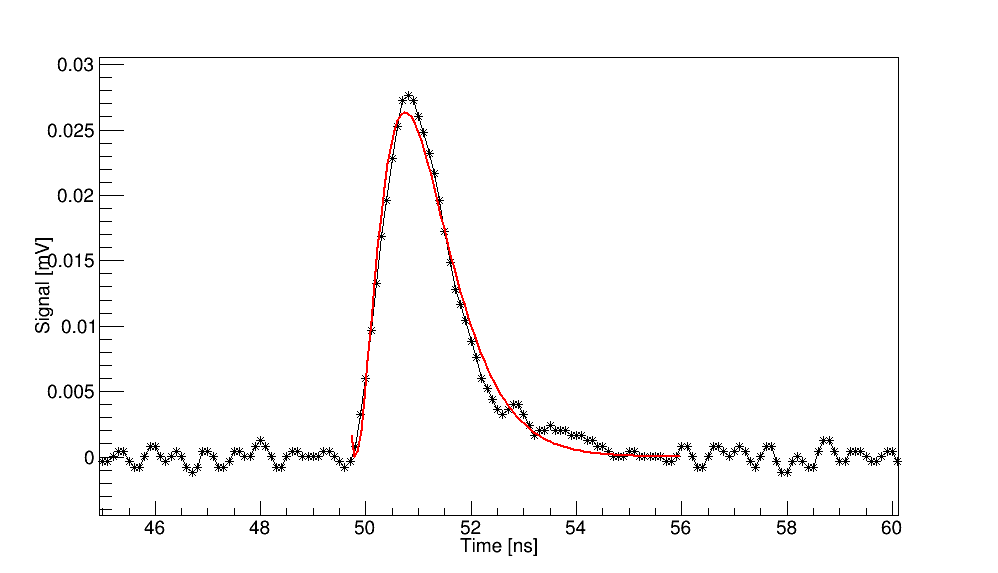
\includegraphics[width=\linewidth]{1pesignalexp.png}
	\captionof{figure}{Анализ формы одноэлектронного шумового сигнала}\label{ris:1pesignalexp}
\end{figure}

Были обработаны десятки таких сигналов, из которых было рассчитано среднее $\bar{b}=0.45$, которое использовалось в моделировании эксперимента в \er.
В~результате моделирования эксперимента с прототипом NeuRad в \er\, были получены формы сигналов, визуально похожие на те, которые мы видели в эксперименте, см. Рис.~\ref{ris:compare}.
С помощью суммарной формы сигнала, Рис.~\ref{ris:integralSim}, был оценено время высвечивания сцинтиллятора как 6\,нс. Таким образом наблюдаем хорошую сходность как качественную так количественную с экспериментальными данными (см. Рис.~\ref{ris:integralform})

\begin{figure}[!ht]
	\centering
	\begin{tabular}{cc}
		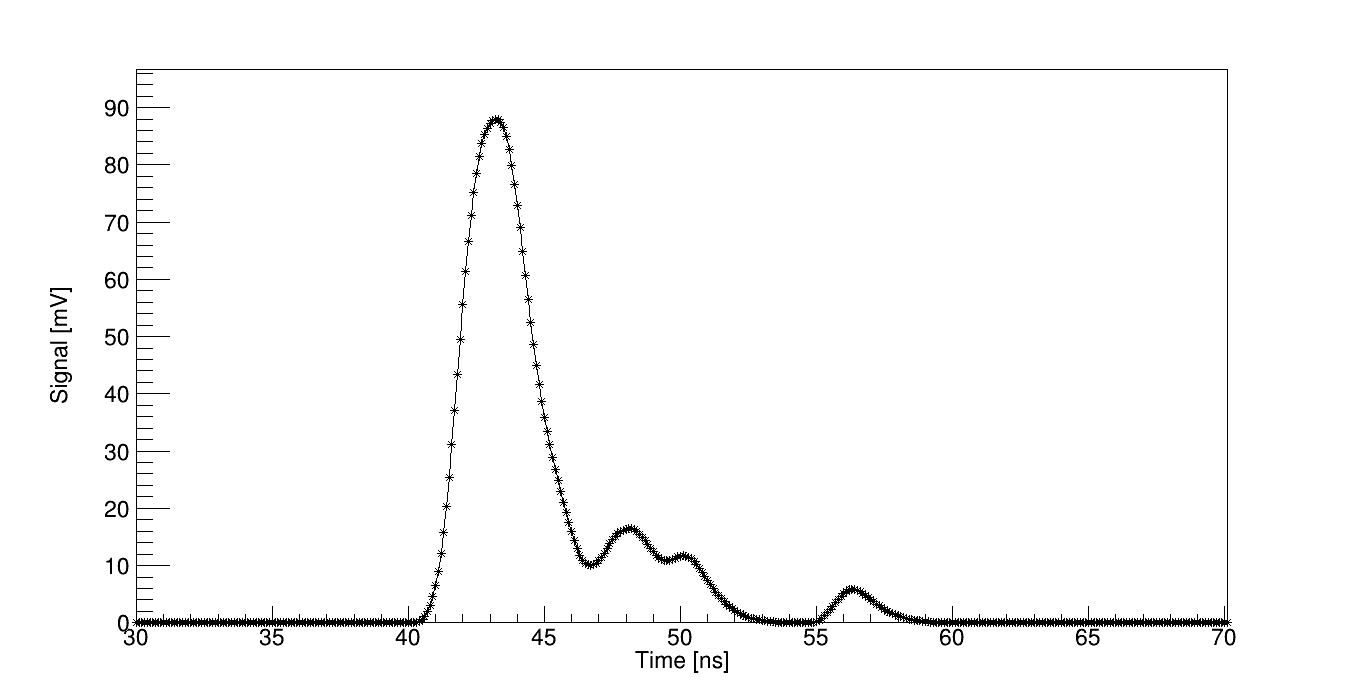
\includegraphics[width=0.52\linewidth]{simSignal1.png} 
		&
		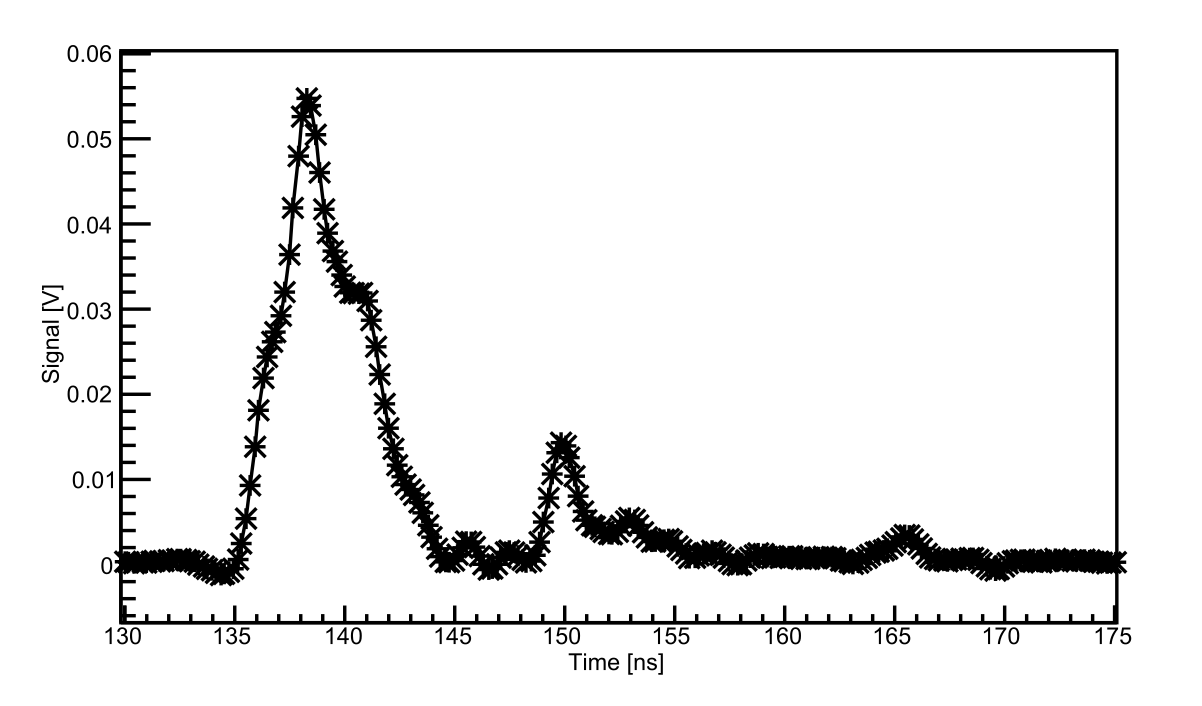
\includegraphics[width=0.48\linewidth]{originalsignalform.png} \\
		а) & б)
	\end{tabular}
	\caption[Short caption for list of figures]{а) Типичный сигнал записанный фреймворком \er\ при симуляции эксперимента с прототипом  NeuRad. б) Типичный сигнал записанный осциллографом в эксперименте.}
	\label{ris:compare}
\end{figure}

\begin{figure}[!ht]
	\centering
	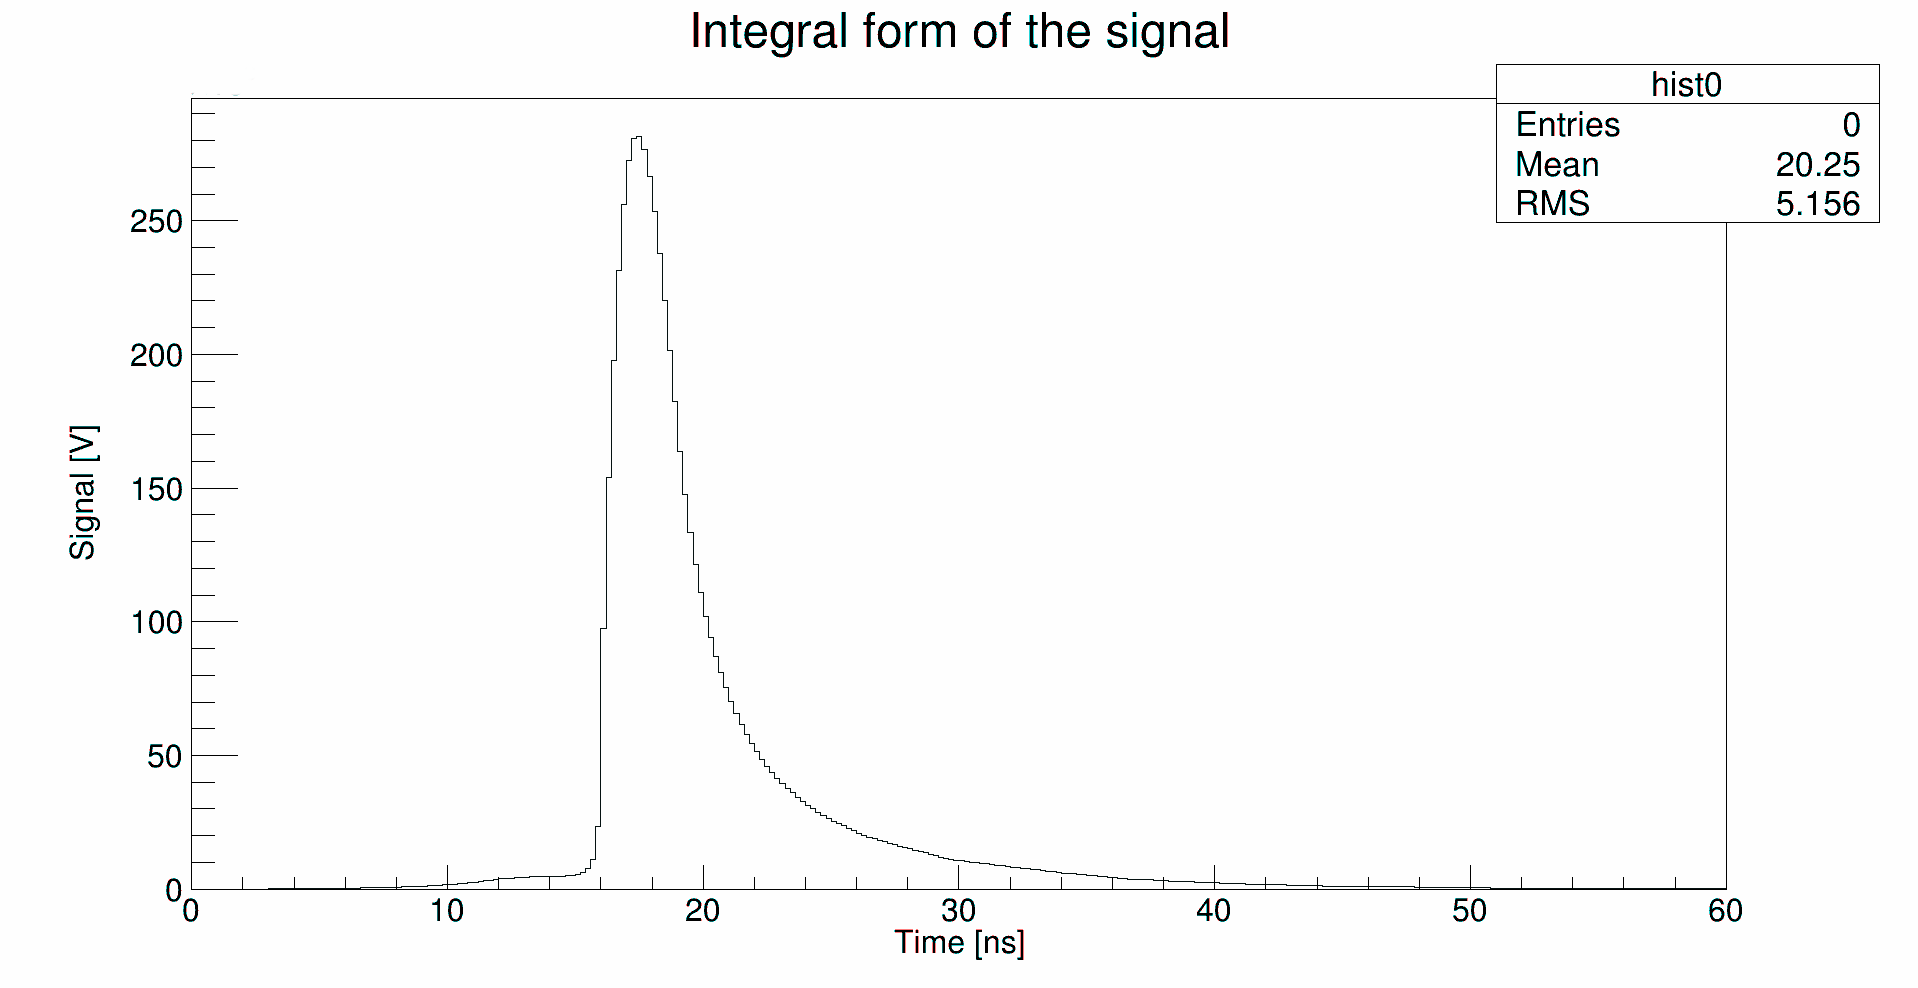
\includegraphics[width=0.8\linewidth]{integralSim.png}
	\caption{Суммарная форма сигналов анода в \er}
	\label{ris:integralSim}
\end{figure}

К полученным в результате моделирования эксперимента сигналам были применены такие же алгоритмы обработки, внедрённые в \er. 
%
Результаты обработки данных с виртуального эксперимента были схожи с результатами обработки экспериментальных данных. На Рис.\ref{ris:tausim} показано сравнение распределений $\Delta\tau$ полученных из экспериментальных и моделированных данных. Времена сигналов в данном случае рассчитывались методом анализа переднего фронта сигнала и равнялись временем превышения передним фронтом сигнала значения, равного половине амплитуды первого локального максимума.

\begin{figure}[!ht]
	\centering
	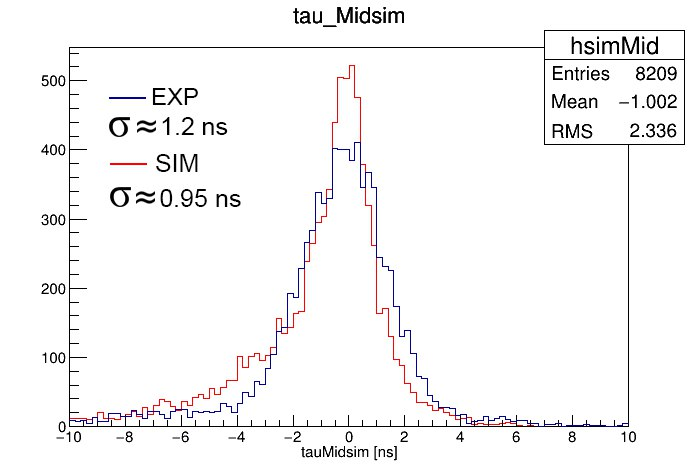
\includegraphics[width=0.8\linewidth]{tausim.png}
	\caption{Распределение $\Delta\tau$ рассчитанное методом анализа переднего фронта для экспериментальных (синим цветом) и моделированных (красным) данных}\label{ris:tausim}
\end{figure}
	
На Рис.\ref{ris:ampsim} изображено сравнение амплитудно-временных корреляций для моделированных, справа, и экспериментальных, слева, данных, где наблюдаем хорошее согласие симуляции с экспериментом. 

\begin{figure}
	\centering
	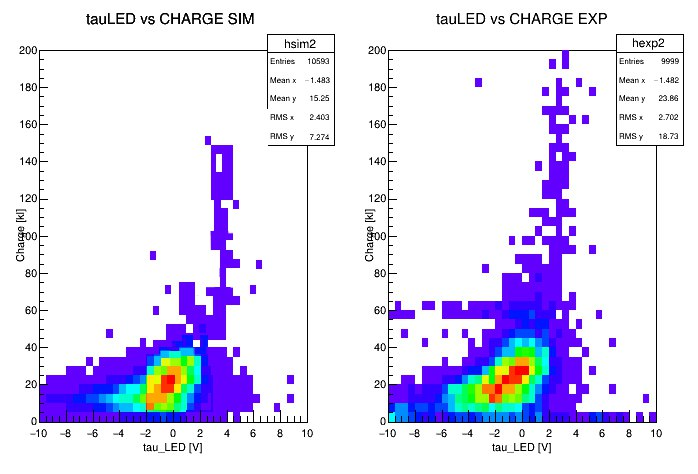
\includegraphics[width=\linewidth]{ampsim.png}
	\caption{Зависимость $\Delta\tau$ рассчитанное методом дискриминатора переднего фронта от заряда. Слева для моделированных, справа для экспериментальных данных }\label{ris:ampsim}
\end{figure}

